\documentclass{standalone}
\usepackage{pgfplots}
\pgfplotsset{compat=newest}

\begin{document}
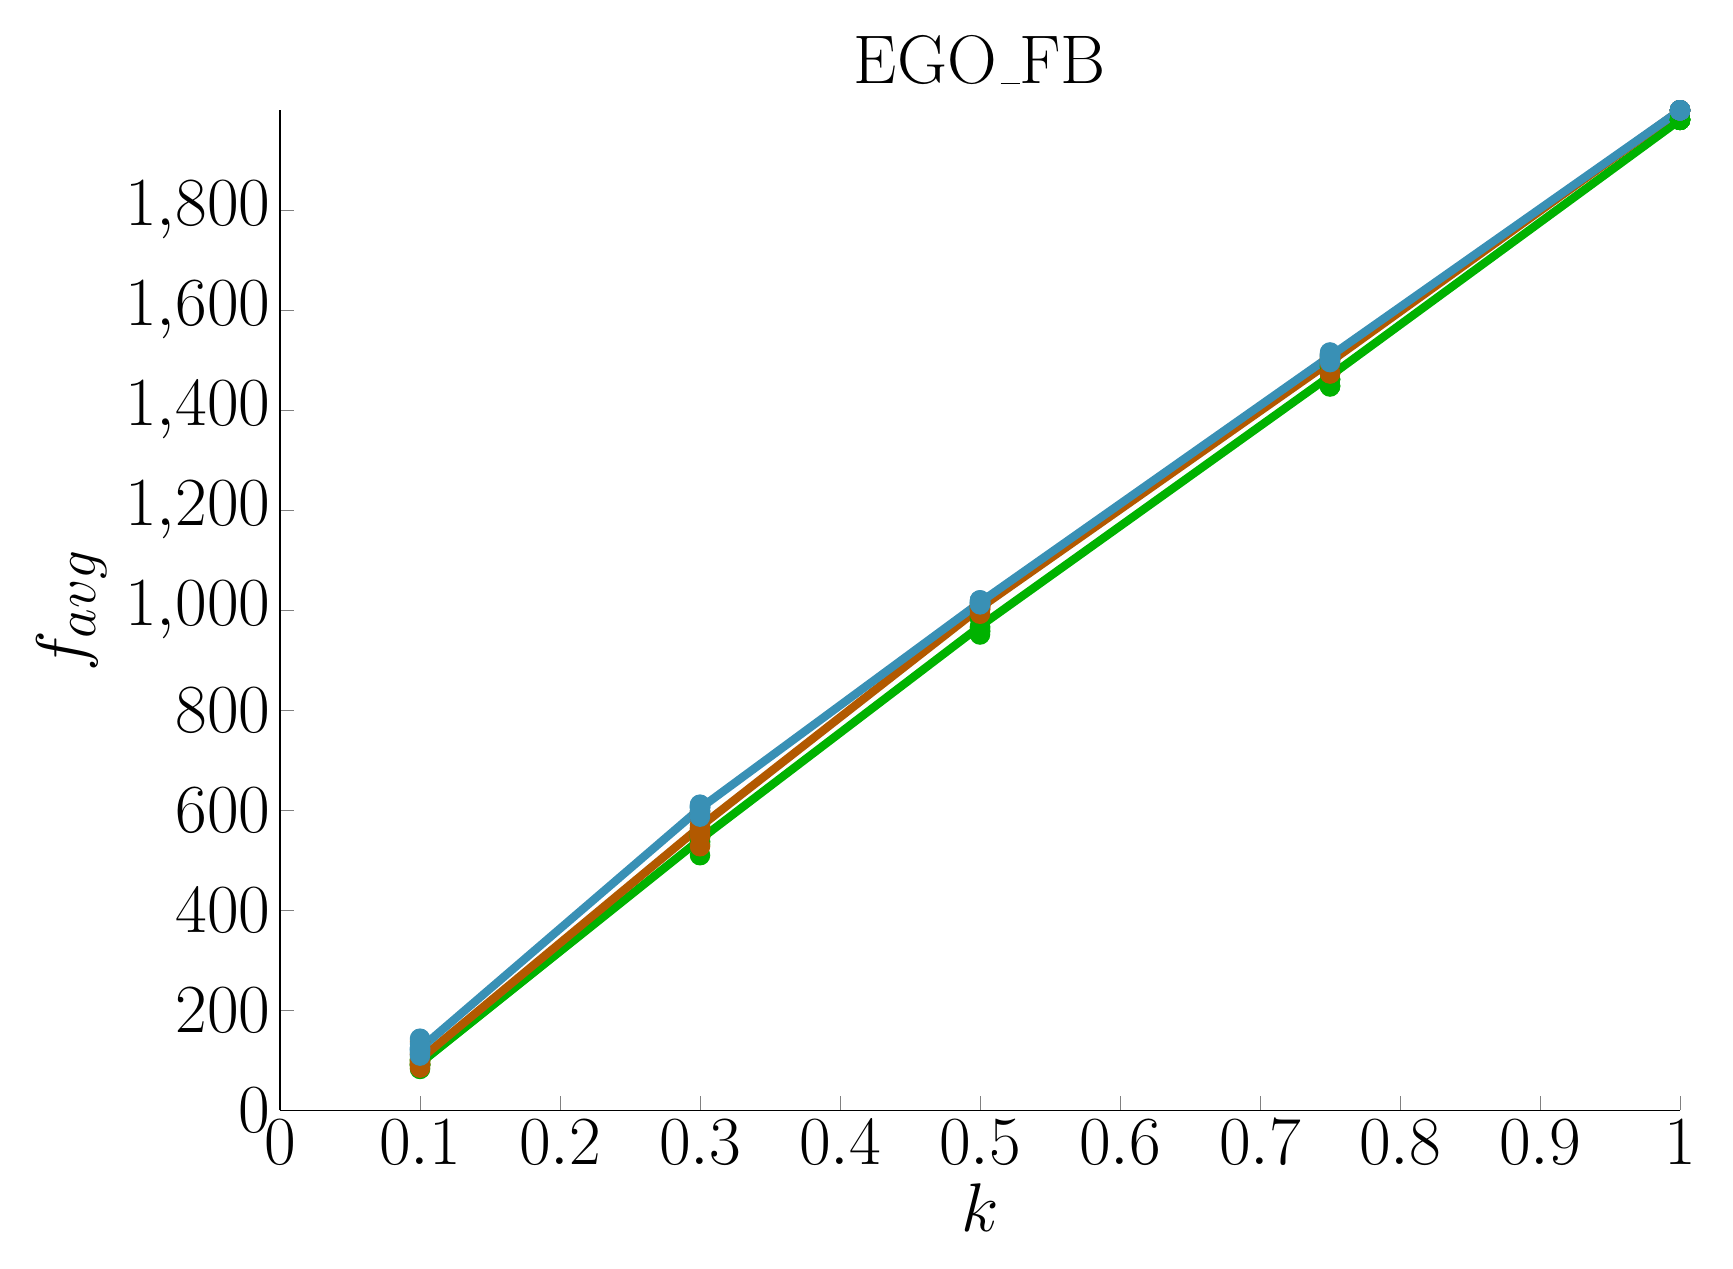
\begin{tikzpicture}

\begin{axis}[%
title style={font=\Huge},
title=EGO\_FB,
tick label style={font=\Huge},
label style={font=\Huge},
legend style={font=\Huge},
view={0}{90},
max space between ticks=50pt,
width=7in,
height=5in,
scale only axis,
xmin=0, xmax=1,
%xtick={0, 20, 40, 60, 80, 100},
xlabel={$k$},
ymin=0, ymax=1999.0,
ylabel={$f_{avg}$},
major tick length=5pt,
axis lines*=left,
legend cell align=left,
clip=false]

\addplot [
only marks,
mark=*,
mark size=3.5pt,
color=green!70!black,
%solid,
%line width=2pt,
]
coordinates{
(0.1,82.64)(0.1,89.58)(0.1,90.38)(0.1,91.62)(0.1,91.64)(0.1,91.68)(0.1,97.14)(0.1,98.92)(0.1,100.48)(0.1,103.28)(0.3,509.88)(0.3,530.84)(0.3,536.2)(0.3,537.44)(0.3,544.84)(0.3,546.66)(0.3,548.88)(0.3,549.8)(0.3,553.46)(0.3,555.44)(0.5,951.08)(0.5,956.7)(0.5,957.64)(0.5,958.82)(0.5,962.72)(0.5,966.0)(0.5,966.82)(0.5,983.76)(0.5,984.84)(0.5,987.4)(0.75,1446.84)(0.75,1447.98)(0.75,1448.46)(0.75,1461.26)(0.75,1461.32)(0.75,1461.32)(0.75,1486.0)(0.75,1486.9)(0.75,1486.96)(0.75,1491.3)(1,1980.0)(1,1980.0)(1,1980.0)(1,1980.0)(1,1980.0)(1,1980.0)(1,1980.0)(1,1980.0)(1,1980.0)(1,1980.0)
};

\addplot [
only marks,
mark=*,
mark size=3.5pt,
color=orange!70!black,
%solid,
%line width=2pt,
]
coordinates{
(0.1,85.36)(0.1,90.32)(0.1,92.12)(0.1,94.04)(0.1,95.42)(0.1,100.04)(0.1,100.54)(0.1,110.4)(0.1,113.38)(0.1,137.48)(0.3,527.84)(0.3,548.16)(0.3,553.66)(0.3,561.26)(0.3,563.24)(0.3,564.3)(0.3,570.36)(0.3,587.6)(0.3,593.16)(0.3,597.44)(0.5,992.62)(0.5,1000.64)(0.5,1001.46)(0.5,1002.96)(0.5,1005.32)(0.5,1007.08)(0.5,1007.32)(0.5,1008.62)(0.5,1008.68)(0.5,1009.7)(0.75,1472.98)(0.75,1473.08)(0.75,1491.82)(0.75,1496.9)(0.75,1499.66)(0.75,1501.6)(0.75,1502.04)(0.75,1503.82)(0.75,1506.5)(0.75,1511.08)(1,1999.0)(1,1999.0)(1,1999.0)(1,1999.0)(1,1999.0)(1,1999.0)(1,1999.0)(1,1999.0)(1,1999.0)(1,1999.0)
};

\addplot [
only marks,
mark=*,
mark size=3.5pt,
color=cyan!70!black,
%solid,
%line width=2pt,
]
coordinates{
(0.1,109.32)(0.1,113.48)(0.1,117.66)(0.1,119.82)(0.1,120.18)(0.1,122.94)(0.1,123.82)(0.1,125.26)(0.1,132.58)(0.1,143.24)(0.3,587.02)(0.3,598.52)(0.3,598.64)(0.3,604.28)(0.3,605.26)(0.3,605.52)(0.3,606.54)(0.3,608.62)(0.3,609.34)(0.3,611.04)(0.5,1011.32)(0.5,1013.34)(0.5,1013.48)(0.5,1013.78)(0.5,1013.88)(0.5,1015.22)(0.5,1015.42)(0.5,1017.76)(0.5,1019.26)(0.5,1019.6)(0.75,1495.58)(0.75,1501.68)(0.75,1504.72)(0.75,1506.92)(0.75,1507.76)(0.75,1508.46)(0.75,1509.52)(0.75,1510.7)(0.75,1512.46)(0.75,1515.02)(1,1999.0)(1,1999.0)(1,1999.0)(1,1999.0)(1,1999.0)(1,1999.0)(1,1999.0)(1,1999.0)(1,1999.0)(1,1999.0)
};
p
\addplot [
color=green!70!black,
solid,
line width=3pt
]
coordinates{
(0.1,93.736)(0.3,541.344)(0.5,967.578)(0.75,1467.834)(1.0,1980.0)
};

\addplot [
color=orange!70!black,
solid,
line width=3pt
]
coordinates{
(0.1,101.91)(0.3,566.702)(0.5,1004.44)(0.75,1495.948)(1.0,1999.0)
};

\addplot [
color=cyan!70!black,
solid,
line width=3pt
]
coordinates{
(0.1,122.83)(0.3,603.478)(0.5,1015.306)(0.75,1507.282)(1.0,1999.0)
};


\end{axis}
\end{tikzpicture}
\end{document}
